\documentclass[a4paper, titlepage, 12pt]{article}
\usepackage[a4paper, margin=2.2cm]{geometry}
\usepackage[utf8]{inputenc}
\usepackage{float, amssymb, amsmath, amsbsy} 
\usepackage{mathdots, mathrsfs, topcapt, multirow}
\usepackage[hidelinks]{hyperref}
\usepackage{graphicx, caption, booktabs}
\usepackage{subfigure}
\usepackage[spanish, es-tabla]{babel}
\usepackage{mathtools, fancyref}
\usepackage{multicol}
\usepackage[x11names,table]{xcolor}
\usepackage{listings}
\usepackage{tikz}
\usepackage{multicol}
\usepackage{amsthm}
\def\proof{\paragraph{Demostraci\'on:\\}}
\def\endproof{\hfill$\blacksquare$}

\newtheorem{thm}{Teorema}[section]


\theoremstyle{definition}%Pone en letra negrita la palabra proposicion,etc 

\newtheorem{de}[thm]{Definición}
\newtheorem{nota}[thm]{Nota}
\newtheorem{ej}[thm]{Ejemplos}
\newtheorem{reco}[thm]{Recordatorio}
\newtheorem{com}[thm]{Comentario}



\theoremstyle{Teorema}   

\newtheorem{prop}[thm]{Proposición}
\newtheorem{teo}[thm]{Teorema}
\newtheorem{coro}[thm]{Corolario}
\newtheorem{lema}[thm]{Lema}
\newtheorem{obs}[thm]{Observación}



\theoremstyle{break}

\newtheorem{demo}{Demostración} % (no lo uso...solo era para probar)


\title{\textbf{Fibonacci Heap aplicado al algoritmo de Dijkstra y Prim}\\
  \vspace{2.5cm}
  \textsc{Facultad de Ciencias, UNAM}\\
  \normalsize\textsc{Programación Declarativa, 2021-1}
}

\author{ Villegas Salvador Kevin Ricardo }

\begin{document}
\maketitle

Como proyecto final se quiere mostrar la utilidad de los montículos de Fibonacci (Fibonacci Heap)
aplicado al algoritmo de Dijkstra para encontrar la ruta mas corta entre dos vértices, al igual que 
aplicado al algoritmo de Prim para encontrar el árbol mínimo.\\

Se mostraran caraccterísticas que hacen a los Fibonacci Heap eficientes por el tiempo amortizado que 
llevan sus funciones. Así poder ver la comparación que tienen al usar alguna Priority Queue a un Fibonacci Heap. 
Se verá la implementación desde leer un archivo \textit{.txt} con el contenido de la representación 
de una gráfica conexa con sus respectivos pesos en la aristas, hasta el proceso de la información para obtener 
el árbol mínimo (Algoritmo de Prim) y la ruta mas corta entre dos vértices(Algoritmo de Dijkstra)

\section{Preliminares}

\subsection{Algoritmo Dijkstra}
El algoritmo Dijkstra, nombrado así por su creador Edsger Wybe Dijkstra (1930-2002), es un algoritmo para 
encontrar el camino mas corto de un vértice a el resto de los vértices de un grafo con pesos en las aristas. 
El algoritmo consiste en ir explorando todos los caminos posibles de un vértice $v_i$ a un vértice $v_j$, 
y de éstos caminos tomar el de peso mínimo.\\

Ya que de un vértice $v_i$ a un vértice $v_j$ tiene que ver todos los caminos posibles, éste vértice $v_i$ 
debe pasar por todos los demás vértices para poder llegar a determinar cual es el camino con peso mínimo.\\

Es por éso que llegamos a que la complejidad del algoritmo es de $O(|V|^2+|E|)=O(|V|^2)$, ahora bien usando 
Priority Queue, llegamos a que la complejidad del algoritmo llega a ser $O((|E|+|V|)\log|V|)=O(|E|\log|V|)$\cite{Complejidad}

\subsection{Algoritmo Prim}
El algoritmo Prim, diseñado por Vojtěch Jarník (1897-1970), después nombrado por así por el cientifico Robert C. Prim, es un 
algoritmo para encontrar el árbol generador mínimo empezando desde un vértice $v_i$ hasta llegar a cada uno de los vértices de 
un grafo conexo con pesos en las aristas.

Ya que de un vértice $v_i$ se debe computar el recubrimiento de llegar a cada uno de los vértices del grafo, 
se debe comparar cada uno de los caminos que hay del vértice $v_i$ a un vértice $v_j$, es decir, sea la arista ($v_i$,$v_j$) la arista 
de peso mínimo, a esta arista se le anexa la arista ($v_j$,$v_k$), siendo ésta otra arista de peso mínimo, para ello se debio comparar con 
el resto de las demás aristas en el grafo. Además se debío seguir el proceso hasta poder tener a todos los vértices del grafo en el árbol 
generador mínimo.\\

Ahora bien siguiendo éste proceso es por lo cual llegamos a que la complejidad del algoritmo es $O(|V|^2)$, sin embargo, si utilizamos 
Priority Queue tenemos una complejidad de $O((|E|+|V|)\log|V|)=O(|E|\log|V|)$\cite{Complejidad Prim}

\subsection{Fibonacci Heap}
Michel L. Fredman y Robert E. Tarjan, en 1987 presentan la estructura de datos Fibonacci Heap, la cual mejora los algoritmos de 
optimización en un flujo de redes.

Un Fibonacci Heap es un bosque de árboles Heap-Ordenados, no siguiendo una estructura definida, es decir, no hay condiciones en el número de 
árboles o su estructura, es parecido a un Heap Binomial sin seguir un orden en especial. La única restricción que siguen los Heap Fibonacci 
son la manera de manipularlos. Ya que es parte de Priority Queue, sigue las operaciones como \textsc{Inserta}, \textsc{Funde}, \textsc{Encuentra mínimo}, 
\textsc{Liga}, \textsc{Borra mínimo}, \textsc{Decrementa llave}, \textsc{Corte en cascada}.\\

Para poder mantener la estructura de un Fibonacci Heap se sigue que:
\begin{itemize}
  \item El propósito de marcar los nodos es guardar la huella por dónde se harán los cortes en cascada.
  \item Tarjan y Fredman generan dos propiedades cruciales:
  \begin{enumerate}
    \item Cada árbol en un Fibonacci Heap no necesariamente es un árbol binomial, pero tiene un tamaño al menos exponencial en el rango de su raíz.
    \item El número de cortes en cascada que durante una secuencia de operaciones está acotado por el número de operaciones que realizan \textsc{Elimina} y 
    \textsc{Decrementa llave}
  \end{enumerate}
  \item La propiedad 1 se basa en lo siguiente:
  \begin{itemize}
    \item \textbf{Lema.} Sea $x$ cualquier nodo en un Fibonacci Heap. Acomodar los hijos de $x$ en el orden en que estos fueron ligados a $x$. Entonces, 
    el $i$-ésimo hijo de $x$ tiene un rango de al menos $(i-2)$.
    \item \textbf{Corolario.} Un nodo de rango $k$ en un Fibonacci Heap tiene al menos: $F_{k+2}$ descendientes, incluyendo el mismo. Donde $F_k$ es el $k$-ésimo 
    número de Fibonacci: $F_0=0$, $F_1=1$, $F_k=F_{k-2}+F_{k-1}$, $k>3$
    \item \textbf{Teorema.} Sea $x$ un nodo en un Fibonacci Heap. Sea $k=rank(x)$.\\
    El tamaño del árbol enraizado en $x$ satisface: $k\geq F_{k+2}$
  \end{itemize}
\end{itemize}

Del \textbf{Corolario} es de donde tenemos el nombre de la estructura Fibonacci Heap, y del comportamiento de la estructura de datos, es que podemos obtner las 
siguientes complejidades.\cite{Amortizado}
\begin{itemize}
  \item \textbf{Inserta.} Se crea un núevo heap, después sólo une el nuevo Heap a la estructura Fibonacci Heap. Ya que ésta operación 
  ocupa la operación \textsc{Funde}, la misma que requiere tiempo constante, \textsc{Inserta} gasta tiempo $\Theta(1)$
  \item \textbf{Funde.} Combina dos Heaps, verifica cual de las dos raíces es menor, de ahí se agrega los árboles de un heap a otro, como solo 
  consta de la asignación, ésta acción requiere tiempo constante.
  \item \textbf{Encuentra mínimo.} Ya que se tiene asignado el árbol mínimo, ésta acción requiere de tiempo $O(1)$
  \item \textbf{Liga.} Sean dos Heaps del mismo rango, ahora bien, se verifíca cual es la raíz mínima seguido se crea un nuevo Heap el cual tiene la raíz mínima 
  seguido de la unión de los hijos de ambos Heaps. Como son sólo asignaciones, se requiere de un tiempo $O(1)$
  \item \textbf{Elimina mínimo.} Se elimina el elemento mínimo del Fibonacci Heap, seguido de, se reorganizan los hijos, ligando aquellos que tienen un mismo rango, 
  hasta que no halla dos Heaps con el mismo rango. De acuerdo al análisis de Tarjan y Fredman, ésta acción requiere de un tiempo total amortizado de $O(\log|V|)$
  \item \textbf{Decrementa llave.} Dado que sólo se cambia el valor de un nodo, y verificar si el nodo padre es marcado o no y solo deslindarlo de la lista de hijos, 
  ésta acción requiere de un tiempo constante.  
\end{itemize}

Dado éstas acciones podemos ver que Fibonacci Heap es muy eficiente a comparación de otros Heaps.\cite{Comparaciones}
\begin{table}[h]
  \centering
  \begin{tabular}{c|cccc}
    \rowcolor{LightBlue2} Operation & Linked list & Binary Heap & Binomial Heap & Fibonacci Heap\\\hline
    Make-Heap & $O(1)$ & $O(1)$ & $O(1)$ & $O(1)$ \\
    Insert & $O(1)$ & $O(\log n)$ & $O(\log n)$ & $O(1)$\\
    Minimum & $O(n)$ & $O(1)$ & $O(\log n)$ & $O(1)$\\
    Extract-Min & $O(n)$ & $O(\log n)$ & $O(\log n)$ & $O(\log n)$\\
    Merge & $O(n)$ & $O(n)$ & $O(\log n)$ & $O(1)$\\
    Decrease-Key & $O(1)$ & $O(\log n)$ & $O(\log n)$ & $O(1)$\\
    Delete & $O(1)$ & $O(\log n)$ & $O(\log n)$ & $O(\log n)$
  \end{tabular}
\end{table}

Para poder ver el tiempo amortizado de la operaciones usamos la función potencial:
\begin{equation*}
  \Phi(H)=t(H)+2\cdot m(H)
\end{equation*}
Donde $t(H)$ son los árboles en el Fibonacci Heap y $m(H)$ son los nodos marcados.\\

Ahora bien, seguimos en los análisis de las operaciones:
\begin{itemize}
  \item \textsc{Inserta}\\
  Sea $H'$ el Fibonacci Heap después de insertar un nuevo nodo.
  \begin{align*}
    \Delta\Phi &= (t(H')+2\cdot m(H'))-(t(H)+2\cdot m(H))\\
    &=(t(H)+1+2\cdot m(H))-(t(H)+2\cdot m(H))\\
    &=t(H)-t(H)+1+2\cdot m(H)-2\cdot m(H)\\
    &= 1 \in O(1)
  \end{align*}
  \item \textsc{Extract-Min}\\
  Dado el costo actual tenemos $O(r(H))+O(t(H))$, donde $O(r(H))$ es el tiempo para fusionar 
  los hijos del árbol raíz, ahora bien, $O(r(n))+O(t(H))$ el tiempo que tarda en actualizar el 
  elemento mínimo, además de consolidar los árboles restantes.
  \begin{align*}
    t(H')\leq r(H) + 1 \text{ ya que dos árboles no tienen el mismo rango}\\
    \Delta\Phi = r(H)+1-t(H) = O(r(H)) \in O(\log n)
  \end{align*}
  \item \textsc{Decrease-Key}\\
  Sea $c$ el número de cortes en cascada, $O(1)$ el tiempo para cambiar la clave y $O(1)$ el tiempo 
  para cortar y añadir el nodo a la lista raíz.
  \begin{align*}
    t(H')=t(H)+c\\
    m(H')\leq m(H)-c+2\\
    \Delta\Phi \leq c+2(-c+2)=4-c \in O(1)
  \end{align*}
\end{itemize}

\subsection{Fibonacci Heap aplicado en el Algoritmo Dijkstra y Prim}
Como ya vimos las complejidades de los algoritmos Dijkstra y Prim, ahora bien, ya que sabemos el timepo 
amortizado con la estructura de datos Fibonacci Heap podemos usar ésta estructura y mejorar el tiempo de complejidad 
de los algoritmos.\\

Sabiendo que los tiempos de la estructura Fibonacci Heap son:
\begin{itemize}
  \item Insertar $O(1)$
  \item Fusionar $O(1)$
  \item Encontrar mínimo $O(1)$
  \item Extraer mínimo $O(\log n)$ tiempo amortizado
  \item Decrementar llave $O(1)$ tiempo amortizado
\end{itemize}

Tenemos el costo de tiempo para los algoritmos de Dijkstra y Prim como:
\begin{align*}
  O(nT_{insertar}+nT_{extract-min}+mT_{decrease-key})\\
  = O(n + n\log n + m)\\
  = O(m + n\log n)
\end{align*}

Que es un tiempo asintóticamente más rápido.

\section{Especificaciones}
Se presentan las herramientas utilizadas para la construcción del sistema,
modulos utilizados para llevar acabo la resolución del problema, así como las pruebas del 
algoritmo.
\subsubsection{Herramientas}
\begin{itemize}
  \item \textbf{Lenguaje de Programación.}\\
  Haskell
  \item \textbf{Sistema de Construcción.}\\
  Cabal (The Common Architecture for Building Applications and Libraries) 2.4.0.0
  \item \textbf{Documentación.}\\
  Haddock 2.22.0
  \item \textbf{Control de versiones.}\\
  GitHub 2.30.0 \href{https://github.com/ciencias-unam/proyecto-final-kevRicardo}{Fibonacci Heap (Dijkstra y Prim)}
\end{itemize}
\subsubsection*{Estructura}
En conjunto con \textbf{Cabal} se realizó la construcción del directorio de la siguiente manera:
\begin{center}
  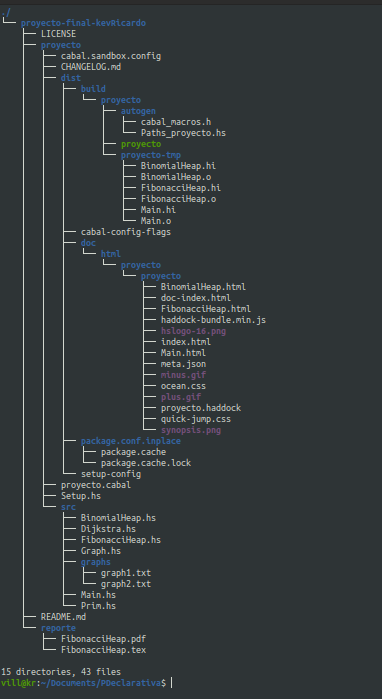
\includegraphics[scale=.5]{img/treepath.png}
\end{center}

Dentro de la carpeta \textbf{./reporte} podemos encontrar, éste archivo. Seguido de la carpeta \textbf{./proyecto} donde 
se encuentra todo lo relacionado con el sistema.\\

Ahora bien seguimos con la siguiente estructura:
\begin{itemize}
  \item \textbf{./dist/build}. Se encuentra el archivo ejecutable.
  \item \textbf{./dist/doc}. La documentación del sistema.
  \item \textbf{./src}. Código fuente
  \item Seguido de la configuraciónes necesarias para poder correr el código
\end{itemize}

\subsection{Manejo del sistema}
\subsubsection*{Descarga del proyecto}
El proyecto se puede encontrar en la siguiente liga: \textit{\href{https://github.com/ciencias-unam/proyecto-final-kevRicardo}{https://github.com/ciencias-unam/proyecto-final-kevRicardo}}. 
Para descargarlo basta con ejecutar \textit{Git} en cualquier directorio del sistema de archivos.\\
\small
\begin{lstlisting}
  $ https://github.com/ciencias-unam/proyecto-final-kevRicardo.git
\end{lstlisting}
\subsubsection*{Compilación y ejecución}
Para poder compilar el proyecto se dará por hecho que ya se tiene \textsc{Cabal} instalado, de lo contrario podrá ejecutar 
\begin{lstlisting}
  $ sudo apt-get install cabal-install
\end{lstlisting}
Una vez ejecutado el comando, podrá ejecutar lo siguiente para poder si \textsc{Cabal} se ha instalado correctamente
\begin{lstlisting}
  $ cabal --version
\end{lstlisting}

Una vez ya teniendo todo listo, podemos comenzar la compilación, y ejecución del programa. Primero nos posicionamos en la ruta
\begin{lstlisting}
  .../PDeclarativa/proyecto-final-kevRicardo/proyecto$
\end{lstlisting}
Ya que estamos en la ruta correcta, para obtener el archivo ejecutable, ponemos el siguiente comando:
\begin{lstlisting}
  .../proyecto-final-kevRicardo/proyecto$ cabal build
\end{lstlisting}
Esto nos generará el ejecutable en la dirección \textit{./dist/buil/proyecto}.
Una vez generado nuestro ejecutable, podemos correr el proyecto con el siguiente comando:
\begin{lstlisting}
  .../proyecto-final-kevRicardo/proyecto$ cabal run
\end{lstlisting}
Cabe mencionar que no es necesario, realizar el ejecutable antes de correr el proyecto, ya que run, lo genera por sí solo.
Para generar la documentación del proyecto, utilizamos el siguiente comando:
\begin{lstlisting}
  .../proyecto-final-kevRicardo/proyecto$ cabal haddock --executables
\end{lstlisting}
Así la documentación la encontramos en \textit{./dist/doc/html/proyecto/proyecto/}\\

Una vez ya corriendo el proyecto empezará por pedir los archivos a procesar para poder probar el algoritmo de Dijkstra y Prim 
usando Fibonacci Heap.

\begin{thebibliography}{99}
  \bibitem{Eficiencia Logaritmica} Herrera S., Salcedo O., Gallego A.. (2014). Efficiency Graphs Algorithmic’s applications oriented to GMPLS networks. Revista Facultad de Ingeniería, 23, 91-104.
  \bibitem{Complejidad} Rodríguez R., Lazo M., (2016). Shortest path search using reduced graphs. Universidad de las Ciencias Informáticas, Facultad 3. Vol. XXXVIII, 32-42
  \bibitem{Complejidad Prim} Rodríguez M., (2009). PROBLEMAS DE OPTIMIZACIÓN EN ÁRBOLES GENERADORES. Tesis de Universidad. UNIVERSIDAD POLITÉCNICA DE MADRID, FACULTAD DE INFORMÁTICA
  \bibitem{Amortizado} M. en I. Gasca M., L. en C. C. Juárez Federico. (2004). El análisis Amortizado y sus Aplicaciones. México: Departamento de Matemáticas.
  \bibitem{Comparaciones} Stajano, F., Sauerwald, T. (2015). Fibonacci Heaps. University of Cambridge, https://www.cl.cam.ac.uk/teaching/1415/Algorithms/fibonacci.pdf
\end{thebibliography}

\end{document}